\section{Hygiene}

Ich mache am Arbeitsplatz eine kleine Sport- oder Strandtasche mit allem nötigen parat (Abb. \ref{fig:sporttasche}).
Glücklich, wer eine eigentliche Garderobe mit abschliessbarem Schrank hat.

Aufhängen der Wäsche im Büro.
Um nasse oder verschwitzte Klamotten kommt man nicht herum.
Schön ist, wenn man diese im Büro aufhängen kann.
Allerdings sollte man die Aversion, die solche Klamotten oder nassen Handtücher auslösen können, nicht unterschätzen.
Was für einem selber die ultimative Trophäe und Beweis seiner Leistungsfähigkeit ist, ist für andere nur eine blanke Zumutung.

\begin{figure}[htpb]
        \centering
        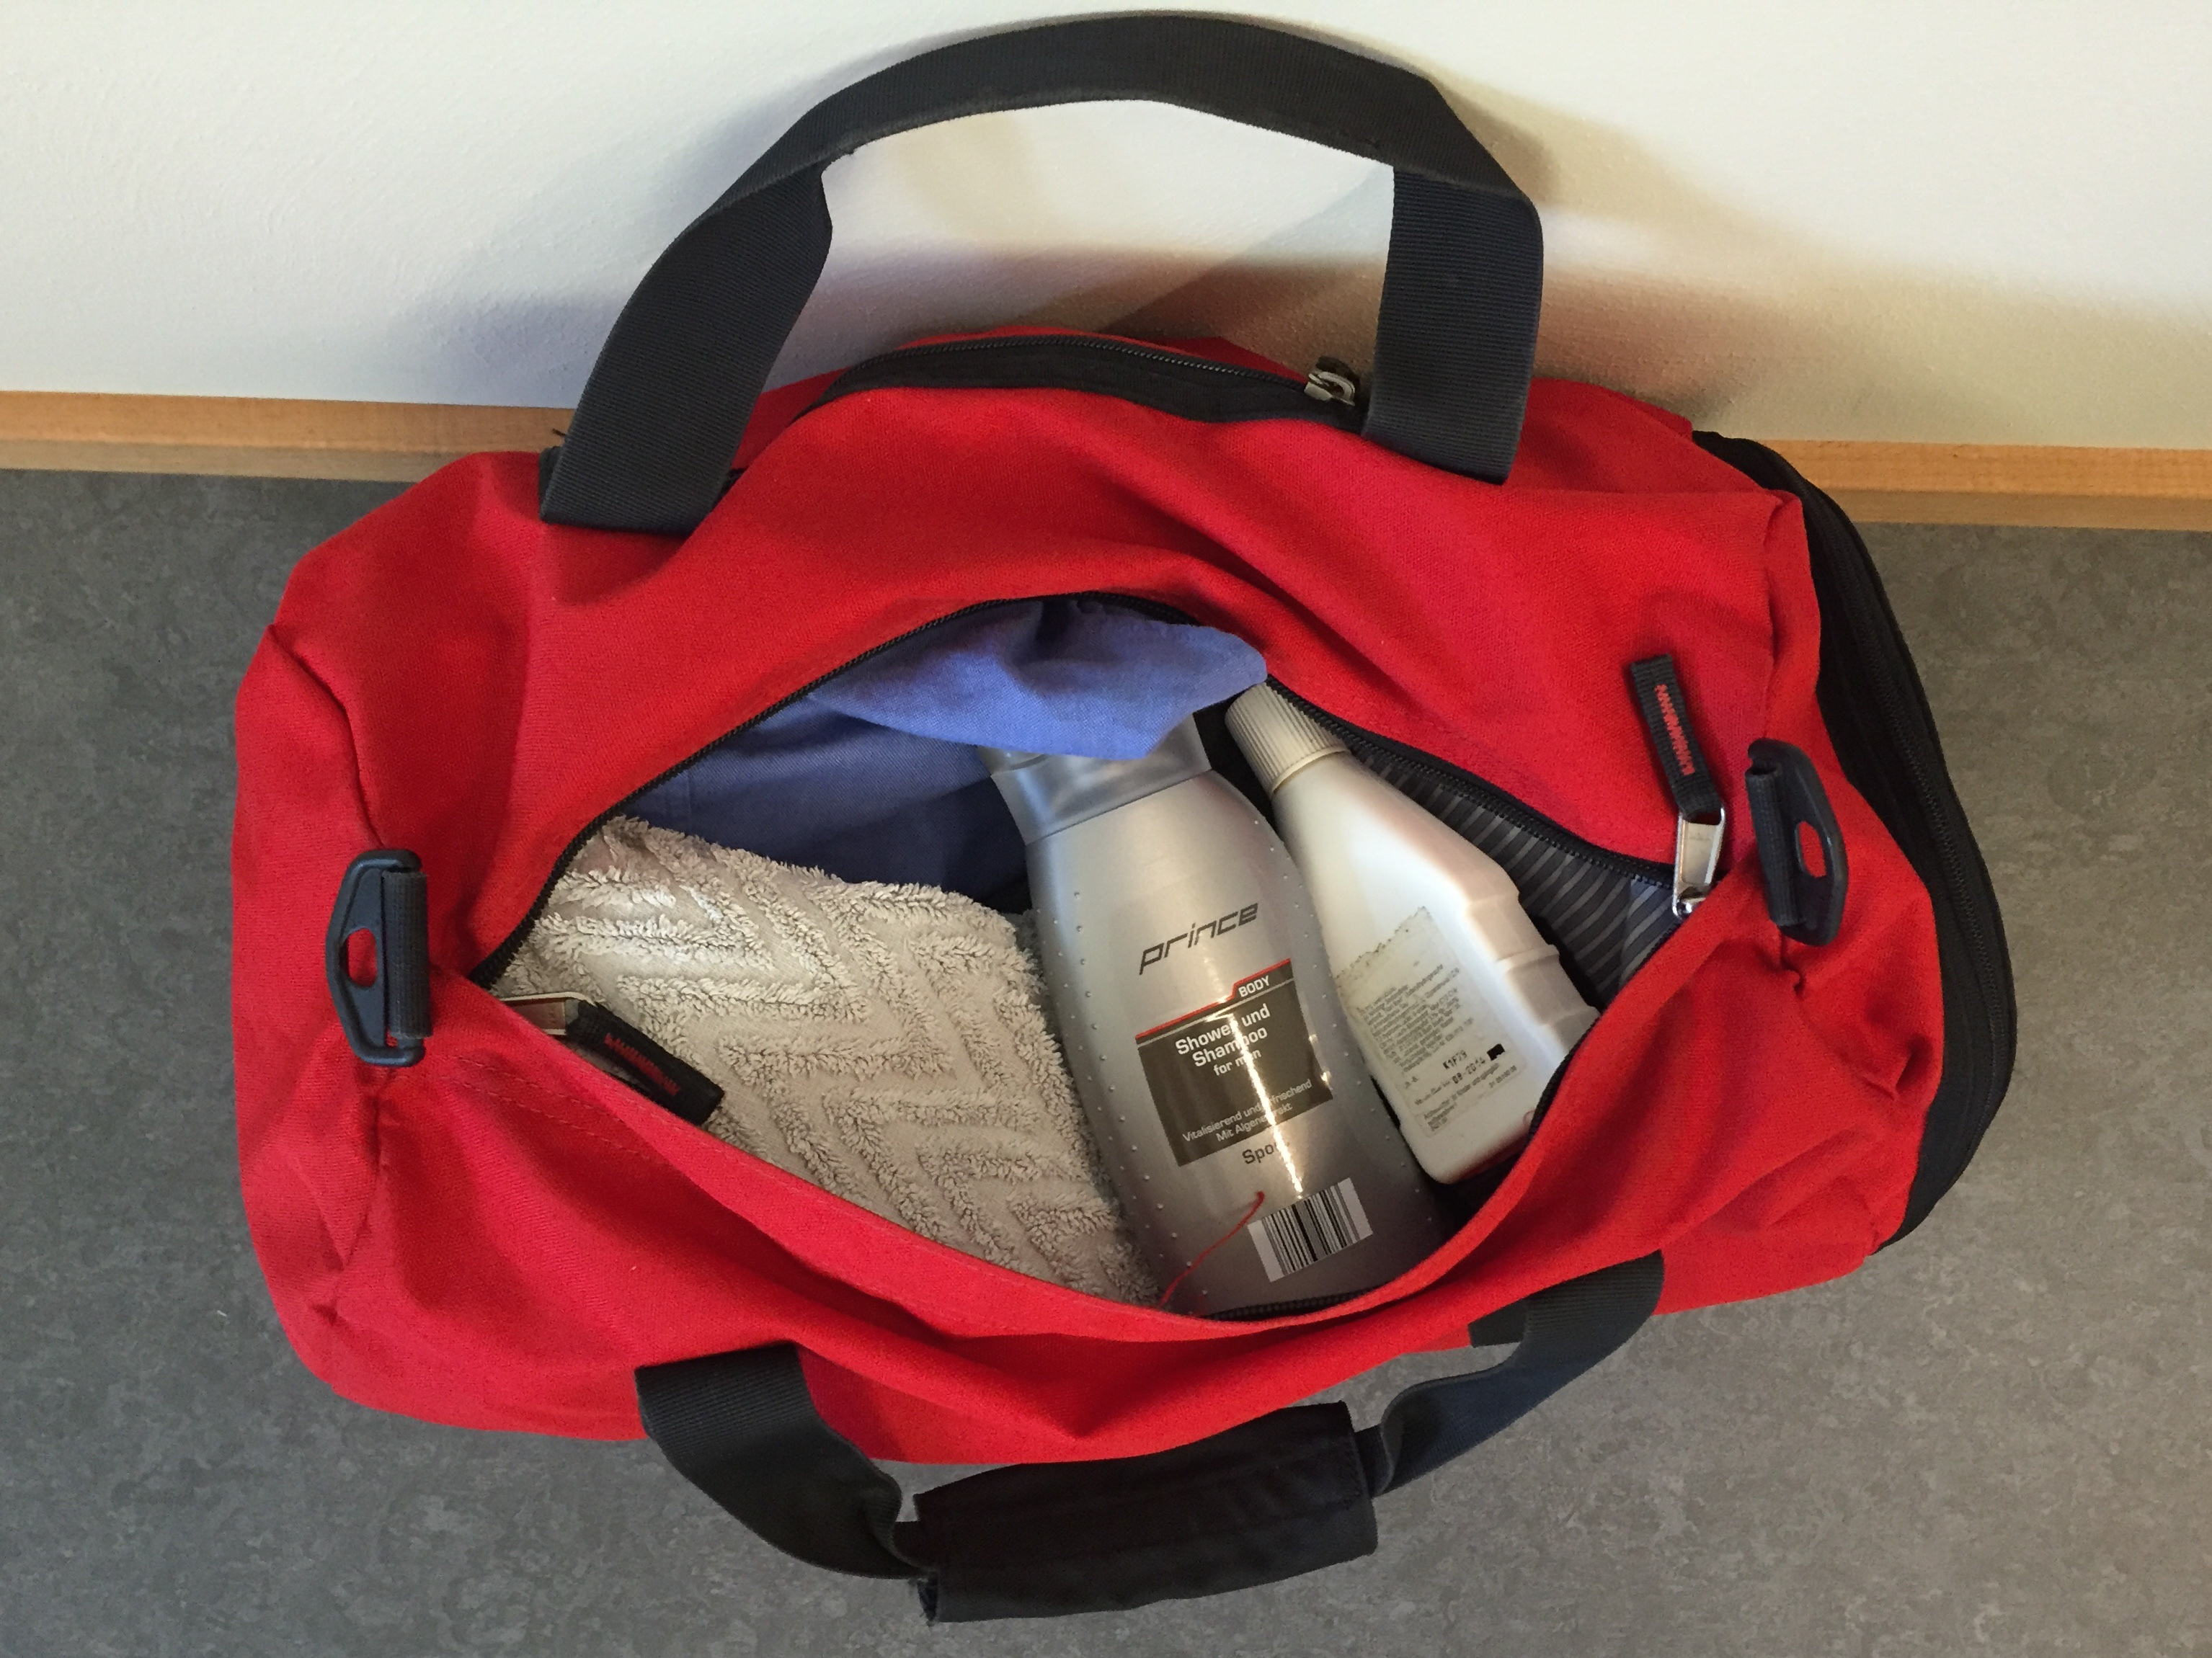
\includegraphics[width=\textwidth]{figures/sporttasche-gepackt.jpg}
        \caption{Im Büro ist eine immer gepackte Sporttasche, in der die Wechselkleider und das Duschzeugs ist.}
        \label{fig:sporttasche}
\end{figure}
